\documentclass[10pt,uplatex]{jsarticle}
\usepackage{amsmath,amssymb,amsthm}
\usepackage{mathtools}
\usepackage[top=2.5cm,bottom=2.5cm]{geometry}
\usepackage[dvipdfmx]{graphicx}
\usepackage{tikz}
\usetikzlibrary{arrows}
\usetikzlibrary{shapes.geometric}
\usetikzlibrary{positioning}
\usepackage{here}
\usepackage{enumerate}
\usepackage{colortbl}
\usepackage{color}
\usepackage{listings}
\usepackage{caption}

\newtheoremstyle{case}{}{}{}{}{}{:}{ }{}
\theoremstyle{case}
\newtheorem{case}{Case}
\usetikzlibrary{intersections, calc, arrows}

\lstdefinestyle{mystyle}{
keywordstyle=\color{magenta},
backgroundcolor=\color{yellow},
commentstyle=\color{green},
basicstyle=\footnotesize,
}
\lstset{style=mystyle}

\title{システム論 中間レポート}
\author{J4-190507 木下裕太}

\begin{document}
    \maketitle

    \section{}
    投票者$v$のShapley-Shubik指数をS$_v$で表すことにし、この値を定義から計算することで各投票者が議決に与える影響力の偏りを見る。投票者の順列であって$A$または$B$が第2項としてピボットとなるものの総数は
    \begin{eqnarray*}
        2!\times3!=12
    \end{eqnarray*}
    であり、残りの第3項がピボットとなる順列のうち$A$または$B$がピボットとなるものの総数は、
    \begin{eqnarray*}
        2\times4!=48
    \end{eqnarray*}
    である。したがって$5$人それぞれのShapley-Shubik指数の値は次のようになる。
    \begin{eqnarray*}
        {\rm S}_A&=&{\rm S}_B=\cfrac{1}{5!}\times\cfrac{12+48}{2}=\cfrac{1}{4}\\
        {\rm S}_C&=&{\rm S}_D={\rm S}_E=\cfrac{1}{3}\times\left(1-\cfrac{1}{4}\times2\right)=\cfrac{1}{6}
    \end{eqnarray*}

    議決のルールや上の考察から直ちにわかることとして以下が挙げられる。
    \begin{enumerate}[(1)]
        \item 役職と影響力が逆転することはなく、同じ役職であれば会議において対等。
        \item 会長$A$と社長$B$が賛成する場合に他の役員の意見が完全に無視される。
        \item 逆に$AとB$の両者が反対したとしても$3$人の役員全員が賛成すれば可決される。
    \end{enumerate}
    通常の会社であれば(1)は当然成り立つべきだろう。
    一方(2),(3)については、議案成立の条件等を考慮しなければ、偏った立場の声が通りやすいということになりflexibleだが慎重さには欠く意思決定になると考えられる。

    \newpage
    \section{}
    消費税率を5,7,9,11\%にするという選択肢をそれぞれ$x_1,x_2,x_3,x_4$とし、$X=\{x_1,x_2,x_3,x_4\}$とする。
    また$n$を正の奇数として投票者を$1,2,\cdots,n$で表し、$V=\{1,2,\cdots,n\}$とする。
    さらに投票者$v$にとっての選好を表す全順序を$>_v$、全体としての選好を表す二項関係を$>_V$とする(後者は順序になるとは限らないことに注意する)。\\
    なお本課題の設定より以下が成り立つことが分かっている。
    \begin{equation}
        |\{v\in V|x_1 >_v x_2\}|,|\{v\in V|x_3 >_v x_4\}|,|\{v\in V|x_1 >_v x_3\}| > \cfrac{n}{2} \tag{☆}
    \end{equation}\\

    まず初めに各投票者の個人選好に制約がない場合を考える。このときnを$3$の倍数として次のように各人の選好を定めることができる。
    \begin{eqnarray*}
        \renewcommand{\arraystretch}{2.5}
        \begin{array}{cc}
            x_1>_v x_3>_v x_4>_v x_2 & if\ 0<v\le\cfrac{n}{3}\\
            x_4>_v x_1>_v x_3>_v x_2 & if\ \cfrac{n}{3}<v\le\cfrac{2}{3}{n}\\
            x_3>_v x_4>_v x_1>_v x_2 & if\ \cfrac{2}{3}n<v\le n
        \end{array}
    \end{eqnarray*}

    これが(☆)を満たすことは容易に確認できる。しかしこのとき
    \begin{eqnarray*}
        x_1>_V x_3\ \land\ x_3>_V x_4\ \land\ x_4>_V x_1
    \end{eqnarray*}
    が成り立ち、$>_V$は推移律を満たさない。
    また最初に比較するペアを$\{x_4,x_1\}$と$\{x_2,x_3\}$などとすれば最終的に$x_4$に決定することになる。
    したがって個人選好が完全に自由であるときには2択ごとの多数決は適切でないと言える。\\

    次に各投票者の選好順序に単峰性を仮定する。
    またより一般の場合を考えるため、代替案の数を4に限定せず$X=\{x_1,\cdots ,x_m\}(\neq\emptyset)$とする。
    つまり次を認めることにする。
    \begin{eqnarray*}
        \forall v\in V, \exists x_{k(v)}\in X\ s.t.\ x_1<_v\cdots<_v x_{k(v)}>_v\cdots>_v x_m
    \end{eqnarray*}
    こうして定まる各$k(v)$に対し、
    \begin{eqnarray*}
        V_l=\{v\in V|k(v)\le l\}
    \end{eqnarray*}
    とする。明らかに$\emptyset=V_0\subset\cdots\subset V_m=V$なので、$n$が奇数であることと合わせて
    \begin{eqnarray*}
        \exists c\in\{1,\cdots,m\}\ s.t.\ |V_{c-1}|<\cfrac{n}{2}<|V_c|
    \end{eqnarray*}
    が言える。この$c$について次ページの補題が成り立つ。
    \newpage
    \newtheorem*{lemma}{Lemma}
    \begin{lemma}
        上で定めた$c$に対し、$\forall x_i\in X,\ i\neq c\Rightarrow x_c>_V x_i$
    \end{lemma}
    \begin{proof}
    mとの大小関係で場合分けして示す。
        \begin{case} $c<i$のとき\\
            定義より
            \begin{eqnarray*}
                V_c\subset\{v\in V\mid x_c>_v x_i\}
            \end{eqnarray*}
            であるから、
            \begin{eqnarray*}
                |\{v\in V|x_c>_v x_i\}|\ge |V_c|>\cfrac{n}{2}
            \end{eqnarray*}
            すなわち$x_c>_V x_i$である。
        \end{case}
        \begin{case} $i<c$のとき\\
            再び定義より
            \begin{eqnarray*}
                V\setminus V_{c-1}=\{v\in V|k(v)\ge c\}\subset\{v\in V|x_i<_v x_c\}
            \end{eqnarray*}
            であるから、
            \begin{eqnarray*}
                |\{v\in V|x_i<_v x_c\}|\ge |V\setminus V_{c-1}|>\cfrac{n}{2}
            \end{eqnarray*}
            すなわち$x_i<_V x_c$である。
        \end{case}
    \end{proof}
    これを踏まえて次の定理を得ることができる。
    \newtheorem*{theorem}{Theorem}
    \begin{theorem}
        $<_V$は$X$上の全順序となる。
    \end{theorem}
    \begin{proof}
        $|X|$についてのinductionによる。$|X|=1$ならば自明だから、以下そうでないCaseを考える。\\
        新たに$X'=X\setminus\{c\}$上の二項関係として$<_V$を$X'$上に制限したものを考え、それを$<_V'$とする。
        各投票者の選好順序を$X'$上に制限したものも単峰性を持つため、inductionの仮定から$<_V'$が全順序であることが従う。
        一方Lemmaよりある$x_c\in X$が存在し、$\forall x_i\in X,\ i\neq c\Rightarrow x_c>_V x_i$であったから、$<_V$も$x_c$を最大元とする全順序になる。
    \end{proof}
    ゆえに単峰性が成り立つならば、この方式で繰り返し投票を行って上位何個かの代替案を選択できることが保証されるため、十分に妥当な意思決定だと言える。

    \newpage
    \section{}
    新型コロナウィルス感染症に関する企業や一般市民の行動について、本レポートでは主に2つの視点から考察していく。

    \subsection{同業種の企業間での自粛期間への対応の差とそれが生む効果}
    ここでは国内の一般企業(Aとする)の目線から、自粛期間中の自社の対応並びにライバル企業(Bとする)の対応がどのような影響を双方に与えるかをゲーム論的な手法で分析したいと思う。\\
    前提として次の3点を明記しておく。
    \begin{enumerate}[(1)]
        \item 企業が自粛期間において今まで通りの体制で継続することは、成員の健康状態への危険性、顧客の減少や消費活動の減衰などの要因によってある程度の不利益を被る。
        \item 自社の休業中に同業種の他社が営業している場合、相対的に損をしてしまう(他社は得をする)。
        \item 両企業は他方の動向を事前に知ることはできず、確率的な選択を行わない純粋戦略をとる。
    \end{enumerate}

    まずはシンプルなモデルとして、表1のような設定を考えてみる。各セルの第1成分はAの損得、第2成分はBの損得を表す数であり、値の大きさや比は特に根拠に基づいていない。

    \begin{table}[h]
        \centering
        \begin{tabular}{c|c|c}
             & B-休業 & B-営業\\\hline
            A-休業 & $-1, -1$ & $-4,0$\\ \hline
            A-営業 & $0,-4$ & $-3,-3$\\
        \end{tabular}
        \caption{2社A,Bの利得関係}
    \end{table}

    上のモデルは囚人のジレンマとよく類似している。
    双方が営業している状態がNash均衡である一方で、パレート最適なのは双方が休業している状態である。\\

    次に利得がパラメータ変数を用いて表される場合について見てみる。休業による損失は本来得られるはずであった顧客の数に依存すると考えられる。
    また顧客はどちらか1社が営業している場合に常に一定数だけ影響を及ぼすとする。これらを加味すると、例えば表2のような設定が可能である。

    \begin{table}[h]
        \centering
        \begin{tabular}{c|c|c}
            & B-休業 & B-営業\\\hline
            A-休業 & $-1, -1$ & $-2x,0$\\ \hline
            A-営業 & $0,-2x$ & $-1-x,-1-x$\\
        \end{tabular}
        \caption{パラメトライズされた2社A,Bの利得関係}
    \end{table}

    このとき$x$と$1$の大小関係によって次のように異なった形で均衡が現れる。
    \begin{itemize}
        \item $x>1$のとき\\
        表1のモデル($x=2$に対応する)と同じNash均衡が存在する。
        \item $x<1$のとき\\
        先の場合とは対照的に、どちらか一方のみ営業している状態がNash均衡となる。
        \item $x=1$のとき\\
        両方休業する以外の3つの状態がNash均衡となる。
    \end{itemize}

    \subsection{急を要する多数の患者の最適な病院への割り当て方法}
    必要とする患者に治療を施すことは国や医療機関の責務であるが、様々な制約やコストが付きまとうためその判断は難しく慎重さを要する。
    ここでは患者と病院のマッチングをどのような基準に沿って決定するべきかを考えてみる。\\

    ここでも前提としていくらか列挙しておく。
    \begin{enumerate}[(1)]
        \item 各患者はいずれも同程度に治療を必要としており、区別なく扱われる。
        \item 患者と病院には地理的な位置が定まっており、両者が離れているほどマッチングのコストは大きい。
        \item 1つの病院に多くの患者が集中することはリスクが高いため避けたい。
    \end{enumerate}

    条件(1),(2)については以下のような2部グラフ(bipartite graph)で表現することができる。
    \begin{itemize}
        \item 各頂点が個々の患者や病院に対応する。
        \item 各辺は患者の病院へのありうる割り当てを示している。またその重みは割り当てのコストに等しい。
    \end{itemize}

    またさらに2つの頂点$s({\rm source}),t({\rm sink})$とそれらに関わる辺を次のように追加したflow network(次ページの図1はその一例)により条件(3)も表現することができる。
    \begin{itemize}
        \item $s$から各患者を表す頂点に容量$1$、コスト$0$の辺を張る。
        \item 先の2部グラフで張った辺に患者側から病院側へと向き付け、容量を1とする。
        \item 各病院から$t$へ向かう、容量をその収容人数、コストを受入れ患者一人あたりの負担とした辺を張る。
    \end{itemize}

    このnetworkにおいて流量を患者数とした$s$から$t$への最小費用流(minimum cost flow)\footnote{$\displaystyle\sum_{e:edge}(eの流量)\times(eのコスト)$が最小となるflowのこと}
    を求めれば、最適な患者受入の分担を知ることができる。
    minimum cost flowは頂点数、辺数および流量についての多項式時間で解けることが知られており\footnote{頂点数$N$,流量$F$の問題に対して$O(FN^2)$で動作するものなどがある}
    、またlinear programmingの特殊ケースとみなして様々なアルゴリズムを適用することもできる。

    \begin{figure}[ht]
        \centering
        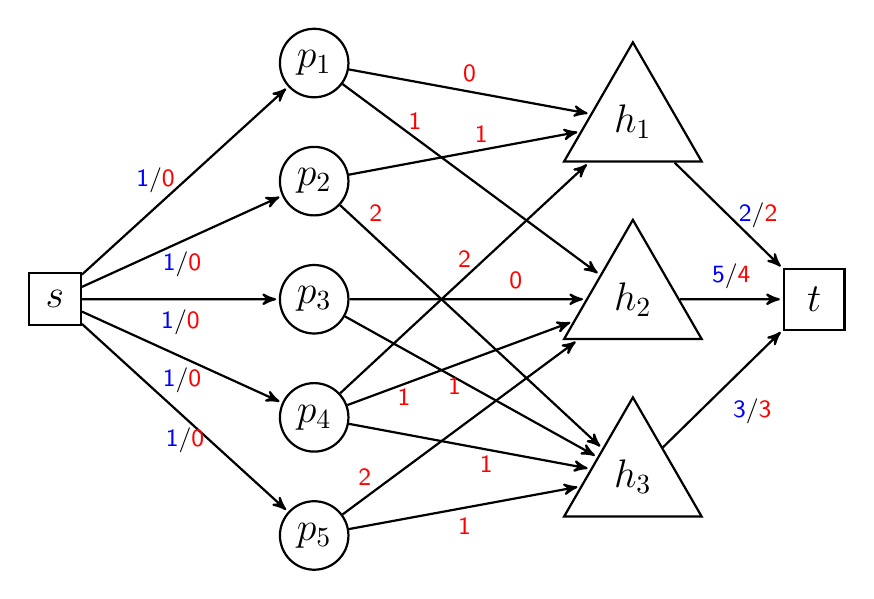
\begin{tikzpicture}[->,>=stealth',shorten >=1pt,auto,node distance=1.5cm,thick,
            square/.style={regular polygon,regular polygon sides=4},
            triangle/.style={regular polygon,regular polygon sides=3},
            pat node/.style={circle,draw,font=\sffamily\Large\bfseries},
            hos node/.style={triangle,draw,font=\sffamily\Large\bfseries},
            ext node/.style={square,draw,font=\sffamily\Large\bfseries}
            ]

            \node[pat node](1){$p_1$};
            \node[pat node](2)[below of=1]{$p_2$};
            \node[pat node](3)[below of=2]{$p_3$};
            \node[pat node](4)[below of=3]{$p_4$};
            \node[pat node](5)[below of=4]{$p_5$};

            \node[hos node](7)[right =3cm of 3]{$h_2$};
            \node[hos node](6)[above=0.7cm of 7]{$h_1$};
            \node[hos node](8)[below=0.7cm of 7]{$h_3$};

            \node[ext node](s)[left=2.5cm of 3]{$s$};
            \node[ext node](t)[right=5.5cm of 3]{$t$};

            \path[every node/.style={font=\sffamily\small}]
            (s) edge node[left]{\textcolor{blue}{1}/\textcolor{red}{0}} (1)
            (s) edge node[below]{\textcolor{blue}{1}/\textcolor{red}{0}} (2)
            (s) edge node[below]{\textcolor{blue}{1}/\textcolor{red}{0}} (3)
            (s) edge node[below]{\textcolor{blue}{1}/\textcolor{red}{0}} (4)
            (s) edge node[below]{\textcolor{blue}{1}/\textcolor{red}{0}} (5)

            (6) edge node[right]{\textcolor{blue}{2}/\textcolor{red}{2}} (t)
            (7) edge node[above]{\textcolor{blue}{5}/\textcolor{red}{4}} (t)
            (8) edge node[below right]{\textcolor{blue}{3}/\textcolor{red}{3}} (t)

            (1) edge node[above]{\textcolor{red}{0}} (6)
            (1) edge node[above left=0.5cm and 0.5cm]{\textcolor{red}{1}} (7)
            (2) edge node[above right]{\textcolor{red}{1}} (6)
            (2) edge node[above left=1.2cm and 1cm]{\textcolor{red}{2}} (8)
            (3) edge node[above right=0.01cm and 0.4cm]{\textcolor{red}{0}} (7)
            (3) edge node[left]{\textcolor{red}{1}} (8)
            (4) edge node[above]{\textcolor{red}{2}} (6)
            (4) edge node[below left=0.2cm and 0.5cm]{\textcolor{red}{1}} (7)
            (4) edge node[below right]{\textcolor{red}{1}} (8)
            (5) edge node[below left=0.4cm and 1cm]{\textcolor{red}{2}} (7)
            (5) edge node[below]{\textcolor{red}{1}} (8);

        \end{tikzpicture}

        \label{fig-1}
        \caption{flow networkの例(各辺のタグは青がcapacity(省略は$1$)、赤がcost)}
    \end{figure}

    \newpage
    参考までにp.7に載せたpythonプログラムは、図1のnetworkに対して最適解(minimum cost flow)を求めるコードであり、実行結果は次のようになる。\\
    \begin{figure*}[h]
        % \centering
        \begin{verbatim}
                        $ python min-cost-flow.py
                        Minimum cost: 17
                        - - -
                        patient -> hospital
                        1 -> 1
                        2 -> 1
                        3 -> 2
                        4 -> 3
                        5 -> 3
                        - - -
        \end{verbatim}
        \captionsetup{labelformat=empty}
    \end{figure*}

    \newpage
    % \begin{quote}
        \begin{verbatim}
    from ortools.graph import pywrapgraph

    pat = 5
    source = 0
    sink = 9

    # Instantiate a SimpleMinCostFlow solver.
    min_cost_flow = pywrapgraph.SimpleMinCostFlow()

    # Add each arc.
    for i in range(pat):
        min_cost_flow.AddArcWithCapacityAndUnitCost(source, i+1, 1, 0)

    min_cost_flow.AddArcWithCapacityAndUnitCost(6, sink, 2, 2)
    min_cost_flow.AddArcWithCapacityAndUnitCost(7, sink, 5, 4)
    min_cost_flow.AddArcWithCapacityAndUnitCost(8, sink, 3, 3)

    start_nodes = [ 1, 1,  2, 2,  3, 3,  4, 4, 4,  5, 5]
    end_nodes   = [ 6, 7,  6, 8,  7, 8,  6, 7, 8,  7, 8]
    unit_costs  = [ 0, 1,  1, 2,  0, 1,  2, 1, 1,  2, 1]

    for i in range(0, len(start_nodes)):
        min_cost_flow.AddArcWithCapacityAndUnitCost(start_nodes[i], end_nodes[i],
                                                    1, unit_costs[i])

    # Add node supplies.
    min_cost_flow.SetNodeSupply(source, pat)
    min_cost_flow.SetNodeSupply(sink, -pat)

    # Find the minimum cost flow between source and sink.
    if min_cost_flow.Solve() == min_cost_flow.OPTIMAL:
        print('Minimum cost:', min_cost_flow.OptimalCost())
        print('- - -')
        print('patient -> hospital')
        for i in range(min_cost_flow.NumArcs()):
            u = min_cost_flow.Tail(i),
            v = min_cost_flow.Head(i),
            f = min_cost_flow.Flow(i)
            if f[0] > 0 and u[0] != source and v[0] != sink:
                print('%d -> %d' % (u[0], v[0] - pat))
        print('- - -')
    else:
        print('Failed to construct flow.')
        \end{verbatim}
    % \end{quote}
\end{document}
